\chapter{Processing of electron backscatter patterns}

Electron microscopes are used in many scientific fields to study microstructure of materials. They rely on electrons instead of photons, which allows them to achieve greater magnification than light microscopes. The microscope emits a beam of electrons, which interact with the specimen, either transmitting through it or reflecting back. The electrons therefore carry an information about the specimen. We capture them on a phosphor screen which emits light and then we take a picture of the screen by a camera, so the result of one electron microscope measurement is an image.

One measurement of electron microscope gets information about only one microscopic point in the specimen. However sometimes we need to map a larger area of the material. For this purpose, scientists use a \emph{scanning electron microscope}. It is a device that repeatedly emits an electron beam towards the specimen, scanning the surface in a raster pattern. So it does the measurement in one place, then moves a bit (e.g. $\SI{1}{\nano\meter}$ aside) and repeats. Since we are measuring the micro world, it takes thousands of iterations to scan a reasonably large area of the specimen. For example, test data that we used for this thesis contained over 15000 images taken in a $120 \times 120$ raster covering an area of the specimen surface approximately $\SI{70}{\nano\meter} \times \SI{70}{\nano\meter}$ big.

In this thesis, we process data obtained using the \emph{electron backscatter diffraction} which is a scientific method that utilizes the scanning electron microscope to study crystalline materials (i.e., materials with a highly ordered microscopic structure). The principle of the electron backscatter diffraction is sketched in \cref{ebsd-principle}. When a beam of electrons is emitted towards the specimen, some of the electrons backscatter, that is, they reflect back from the surface. They are then captured on a phosphor screen which is coupled with compact lens that directs the captured image towards a camera. The result of this procedure is a grayscale image of the \emph{electron backscatter pattern}. An example of such pattern is shown in \cref{roi-shifts:initial}. White color in the image can be interpreted as a place where many electrons were captured whereas black areas captured smaller amount of electrons.

\begin{figure}
	\centering
	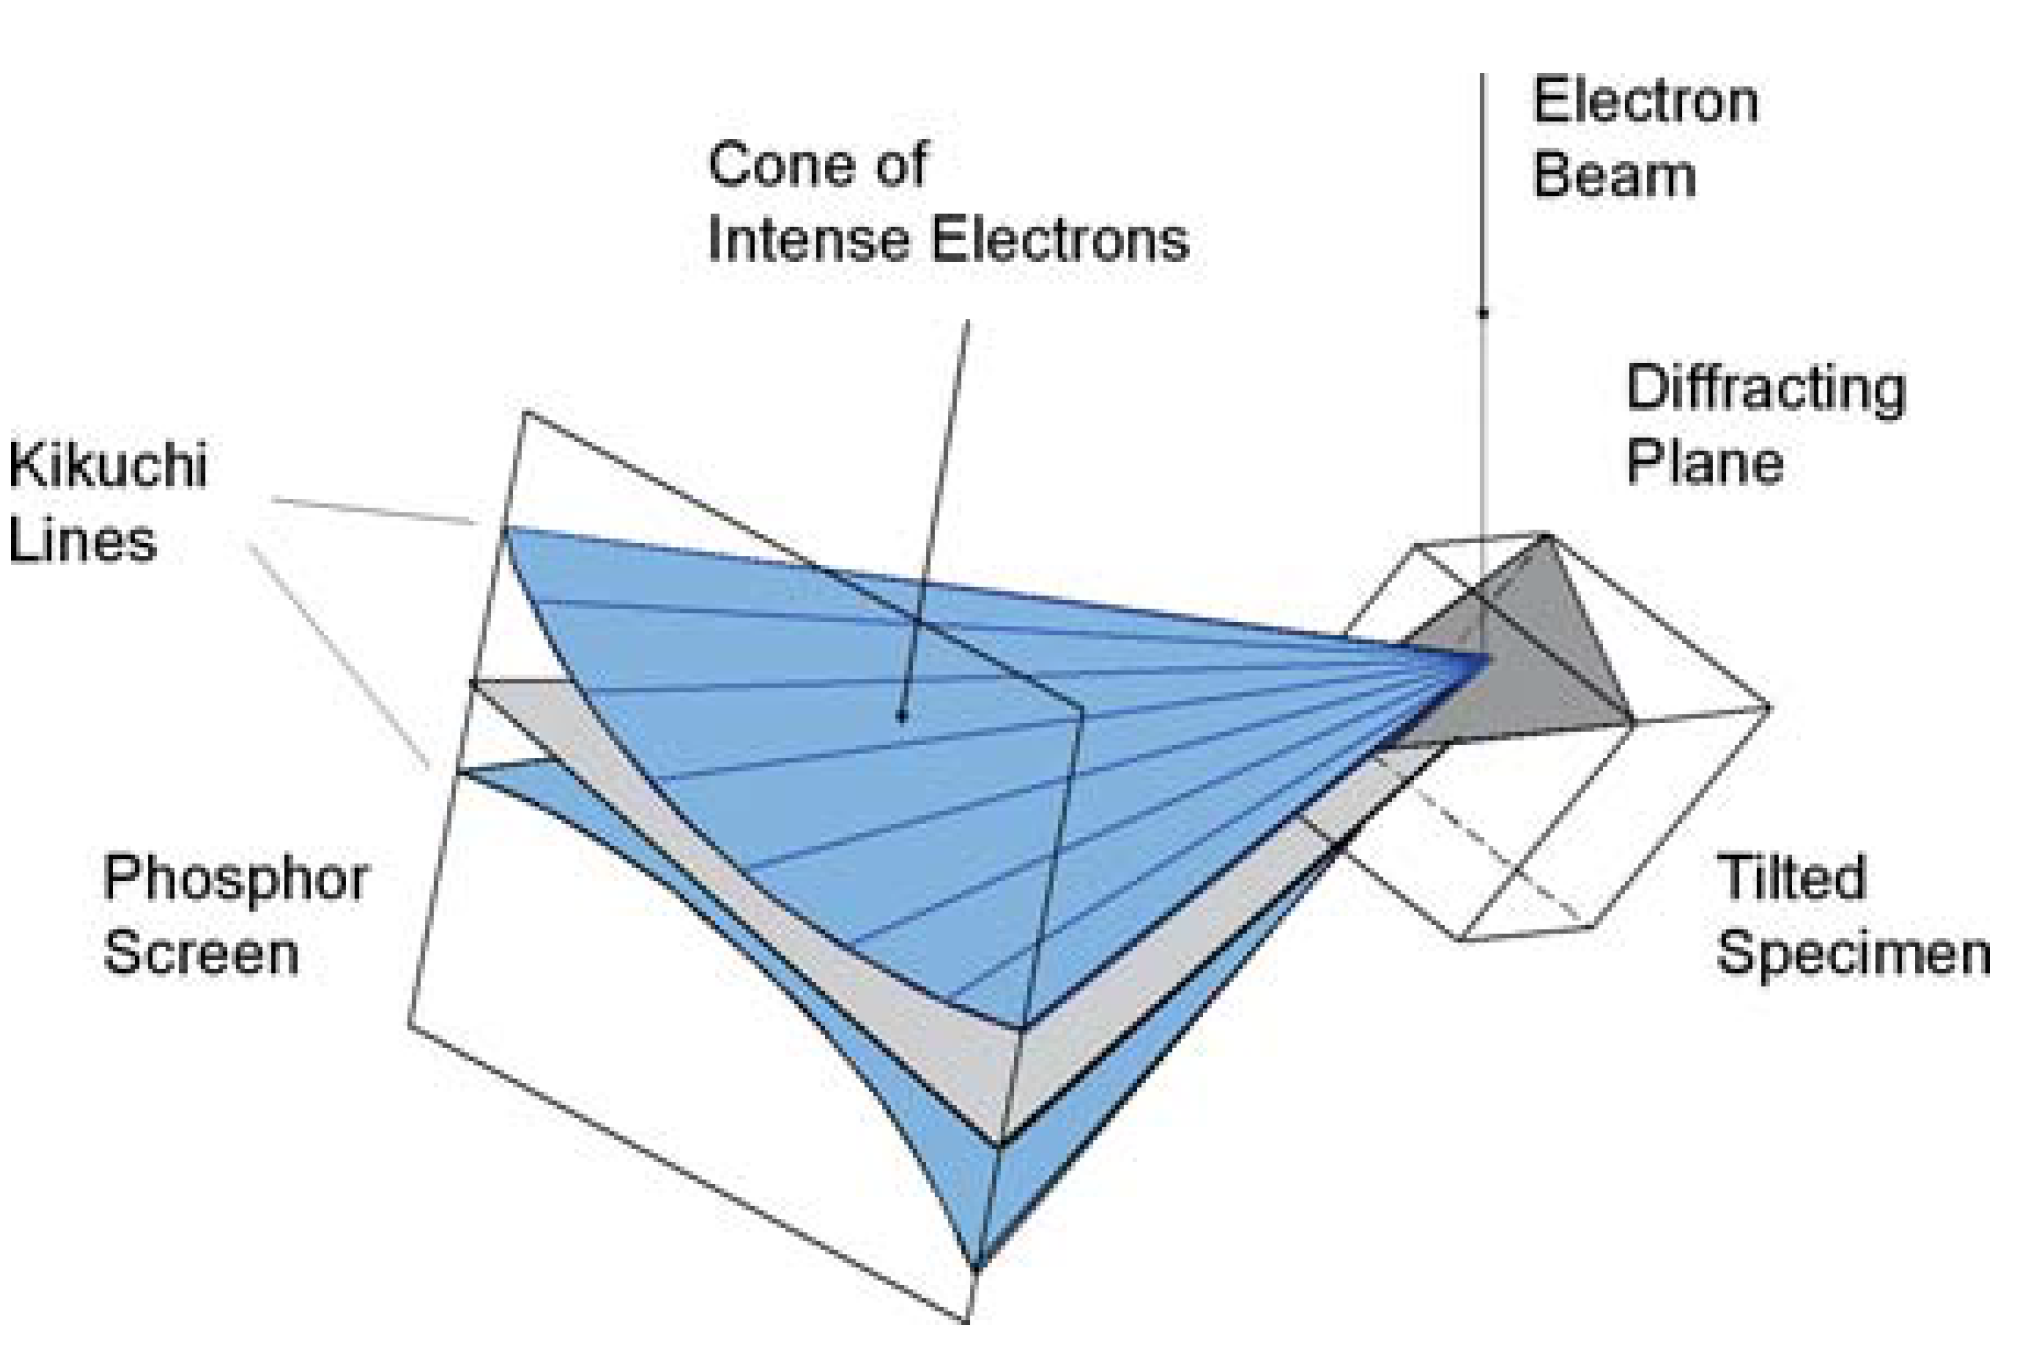
\includegraphics[width=0.6\textwidth]{img/ebsd_principle}
	\caption{The principle of electron backscatter diffraction. \cite{schwartz2009electron}.}
	\label{ebsd-principle}
\end{figure}

\begin{figure}
	
	\begin{subfigure}{.4\textwidth}
		\centering
		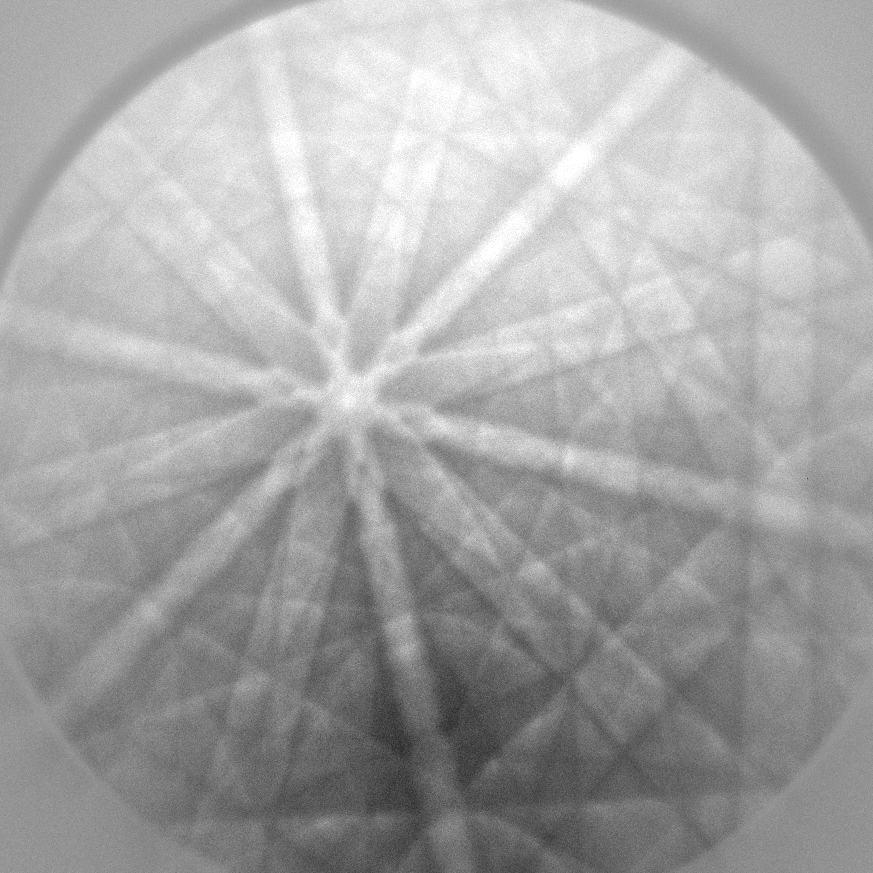
\includegraphics[width=.9\linewidth]{img/roi_shifts_initial}
		\caption{Initial, undeformed pattern}
		\label{roi-shifts:initial}
	\end{subfigure}%
	\begin{subfigure}{.4\textwidth}
		\centering
		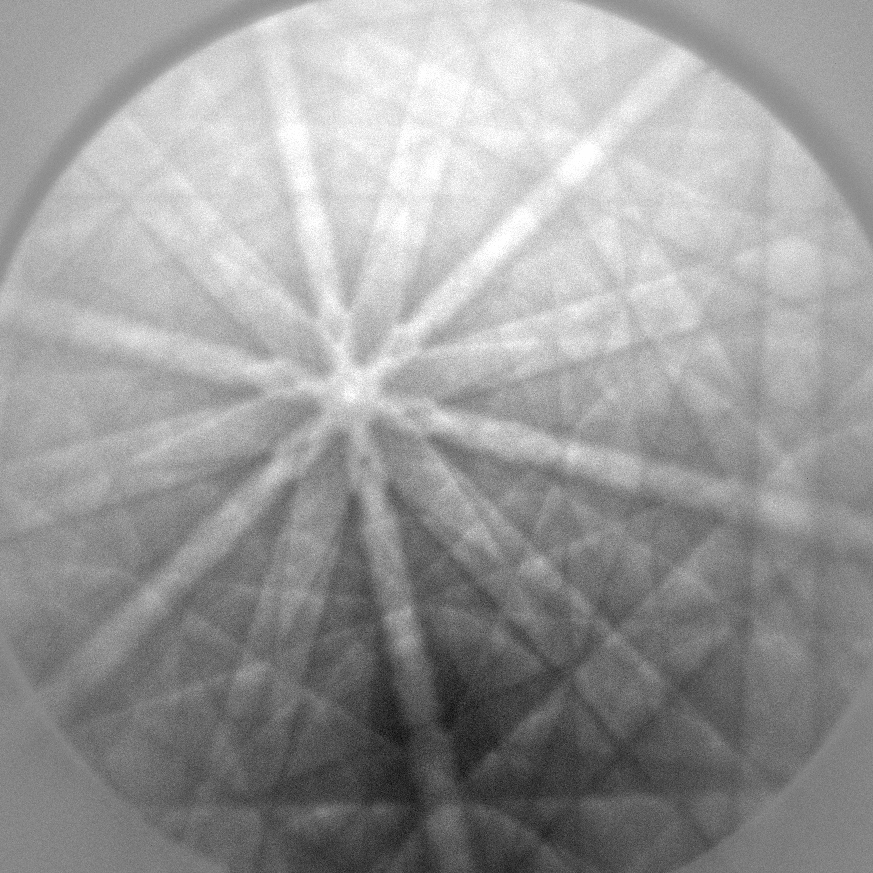
\includegraphics[width=.9\linewidth]{img/DEFORMED_x3600y6235}
		\caption{Deformed pattern}
		
	\end{subfigure}
	\centering
	\begin{subfigure}{.4\textwidth}
		\centering
		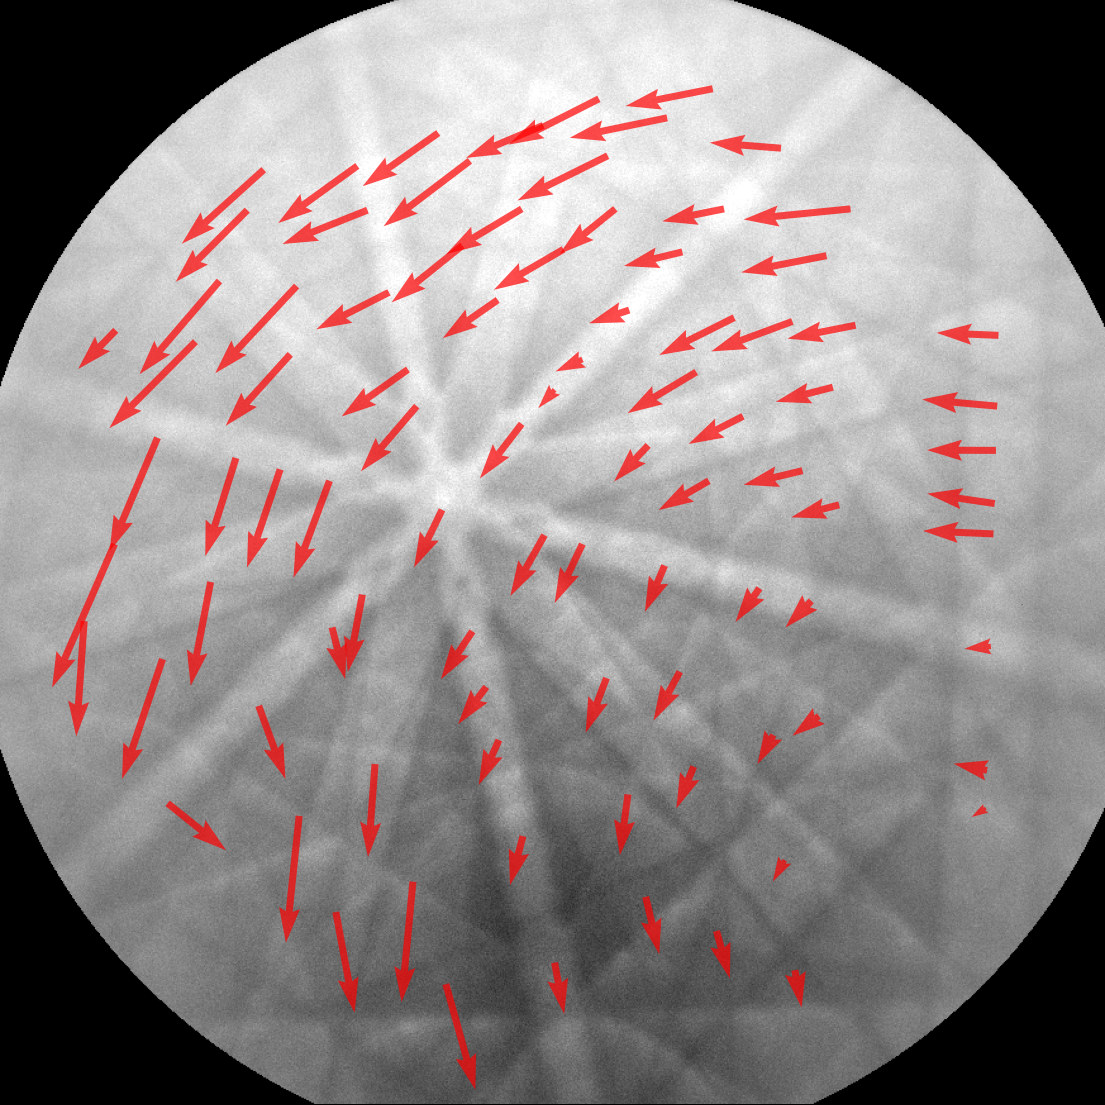
\includegraphics[width=.9\linewidth]{img/roi_shifts}
		\caption{Deformation visualization}
		\label{roi-shifts:result}
	\end{subfigure}
	
	\caption{Deformed pattern with arrows visualizing the deformation. The arrows are upscaled for the visualization, because the pattern is deformed only by several pixels (the biggest offset is less than 10 pixels long, while the whole picture has resolution $873 \times 873$).}
	\label{roi-shifts}
\end{figure}

The electrons do not reflect randomly, but based on the examined specimen, they backscatter in a specific way, forming \emph{Kukuchi lines} observable in the pattern. The geometry of Kukuchi lines can be interpreted as a projection of the specimen crystal structure on the flat phosphor screen.

When the crystal structure of material is changed (e.g. under stress), the deformation can be observed in the backscatter pattern as well. Therefore, the patterns of deformed specimen can be compared to undeformed ones to measure elastic strain and crystal lattice rotation.  \Cref{roi-shifts} shows a visualization of such comparison. Since different parts of the images may be deformed differently, a commonly used technique \cite{wilkinson2006high,wilkinson2010high,britton2012high} is to choose several (usually tens to hundreds) subregions of the patterns and determine the vector of shift between the corresponding regions from both patterns. The shifts estimate the real deformation of the crystalline structure.

The comparison is done by cross--correlating respective subregions of the deformed and reference patterns. The position of the maximum value in the correlation result determines the most probable shift with one pixel precision, which is not enough. To achieve subpixel accuracy, we estimate the peak of the cross--correlation by interpolating from a small neighborhood of the maximum.

Once the shifts are computed, they are further processed to obtain an estimation of the actual crystal deformation and other characteristics. However, we do not address that part of the analysis in this thesis, as it is not nearly as computationally expensive as the processing of the images. Moreover, the comparison is commonly used in analysis of the electron backscatter diffraction data, while the processing of the shifts may be different for various purposes.

To sum up, we have thousands images of deformed electron backscatter patterns. Each of them is captured by a scanning electron microscope at a specific location of a specimen. Moreover, we have one reference image of the electron backscatter pattern. We need to quantify the deformation of each deformed pattern, so we choose several subregions and cross--correlate each respective reference and deformed subregion. Maximal correlation gives us the most probable shifts of the subregions. So for each deformed pattern, the result of our algorithm is a list of shifts corresponding to subregions. The shifts are then further processed to obtain their physical interpretation, but that is not covered in this thesis.

%In this chapter we describe the algorithm used to analyze the deformation of the patterns. We define cross--correlation and least squares --- techniques that are used in the analysis. Finally, we describe the algorithm that we study in this thesis.

\section{Cross--correlation}
\label{cross-corr-def}
Cross--correlation provides a measure of similarity of two series for each possible shift between them. It is used in signal processing to find a shorter known feature in a signal or in image processing to locate a smaller shape in a bigger picture. In analysis of the backscatter patterns, it is used to find the most probable relative displacement between two images (subregions of images).

Cross--correlation of two discrete functions $f$ and $g$ is function $C$ defined as follows:
\[
C[n] = (f \star g)[n] = \sum_{m=-\infty}^{\infty}f[m]g[m+n],
\]
where $\star$ denotes cross--correlation.

If $C = f \star g$ then $C[n]$ is a number that tells us how much are functions $f$ and $g$ similar, when $g$ is shifted by $n$ to the left. For each negative $n$, $g$ is shifted to the right. \Cref{correlation-example} shows two example functions and their cross--correlation.

\begin{figure}
	\centering
	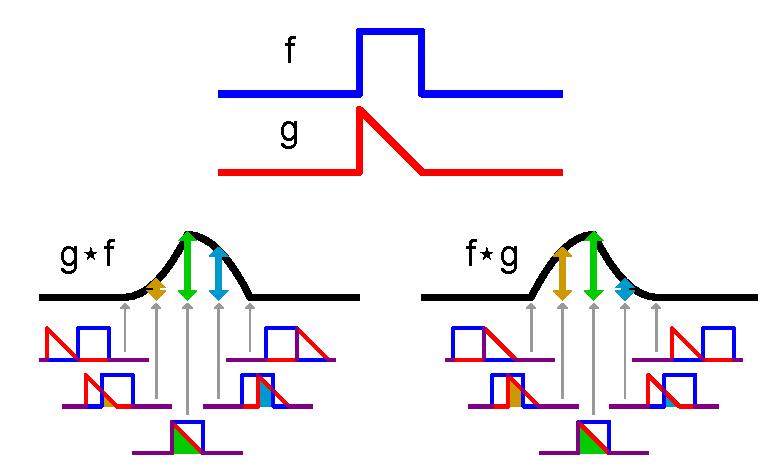
\includegraphics[width=0.7\linewidth]{img/correlation}
	\caption{The cross--correlation of two example functions. The image is taken from \cite{correlation_example}.}
	\label{correlation-example}
\end{figure}

Definition of cross--correlation can be extended for two dimensions. For two--dimensional functions $f$ and $g$, their cross--correlation is defined as:
\[
C[i,j] = (f \star g)[i,j] = \sum_{x=-\infty}^{\infty}\sum_{y=-\infty}^{\infty}f[x,y]g[x+i,y+j].
\]

Analogously to one--dimensional cross--correlation, $(f \star g)[i,j]$ is a number that is higher if $f$ is similar to $g$ shifted by $i$ horizontally and by $j$ vertically. \Cref{2d-correlation-example} demonstrates how cross--correlation can be used to search for a smaller pattern in a bigger picture. The brightest points (maxima) in \cref{2d-correlation-example-result} correspond to the best matches between the pattern and the image.

\begin{figure}
	\centering
		\begin{subfigure}{.49\textwidth}
		\centering
		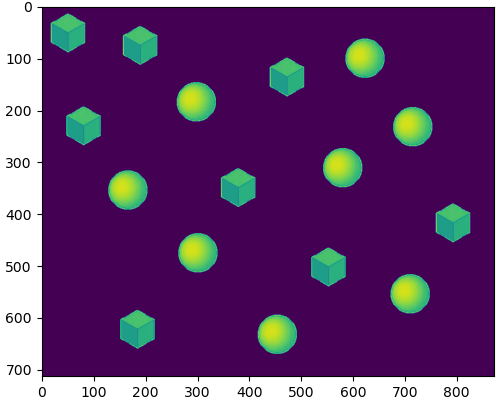
\includegraphics[width=\linewidth]{img/shapes}
		\caption{An image}
	\end{subfigure}
	\begin{subfigure}{.49\textwidth}
	\centering
	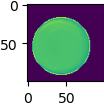
\includegraphics[width=0.4\linewidth]{img/shapes_pattern}
	\caption{Search pattern}
	%\label{fig:sub2}
	\end{subfigure}
	\begin{subfigure}{.5\textwidth}
		\centering
		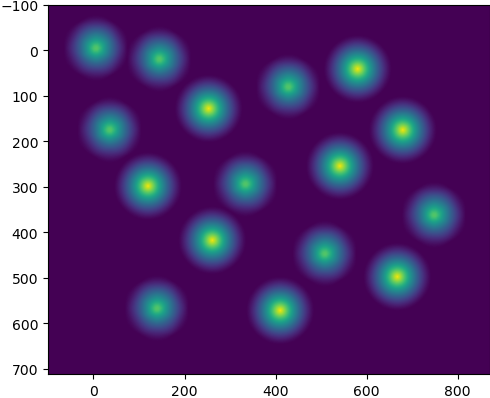
\includegraphics[width=\linewidth]{img/shapes_correlated}
		\caption{Cross--correlation of the (a) and (b) images}
		\label{2d-correlation-example-result}
	\end{subfigure}
	
	\caption{An example of cross--correlation used to find an object in an image. The maxima of the cross--correlation result correspond to the location of the search pattern (b) in the image (a).}
	\label{2d-correlation-example}
\end{figure}

Theoretically, the domain of cross--correlation is whole $\mathbb{Z}^2$. However, when cross--correlating two images, $(f \star g)[i,j]$ does not make sense for too big $i$ or $j$ because the images would be shifted so much they would not overlap. For two images with sizes $w_1 \times h_1$ and $w_2 \times h_2$, the size of their cross--correlation is $(w_1 + w_2 - 1) \times (h_1 + h_2 - 1)$. The result is a rectangle with the following corners: $[-w_1+1,-h_1+1]$, $[-w_1+1,h_2-1]$, $[w_2-1,h_2-1]$, $[w_2-1,-h_1+1]$. Those are the points of cross--correlation, where the result is computed from the images overlapping only by one pixel.

\subsection{Zero--normalized cross--correlation}

Cross--correlation as it is defined in the previous section has a major flaw for image processing: it is heavily affected by the brightness of the images. Consider an image, that has some subregions brighter than others. Then, by definition of cross--correlation, that subregions add more to the result, regardless of the second image. \Cref{normalized-initial} shows an example of an image that is much brighter in the top part then in the bottom. \Cref{normalized-simple-cross} shows the result of cross--correlation with the search pattern in \cref{normalized-pattern}. It is clear that the highest values are located where the original image is brightest instead of locating the search pattern.

\begin{figure}
	\centering
	\begin{subfigure}{.5\textwidth}
		\centering
		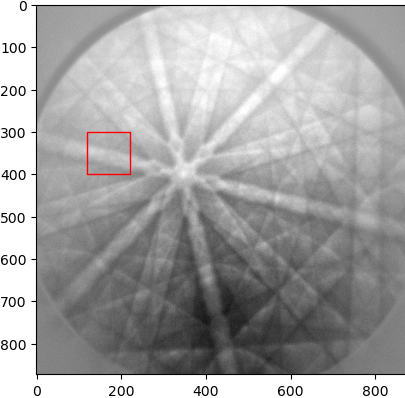
\includegraphics[width=\linewidth]{img/normalized_initial}
		\caption{An electron backscatter pattern}
		\label{normalized-initial}
	\end{subfigure}
	\begin{subfigure}{.4\textwidth}
		\centering
		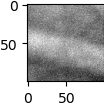
\includegraphics[width=0.4\linewidth]{img/normalized_pattern}
		\caption{Search pattern}
		\label{normalized-pattern}
	\end{subfigure}
	\begin{subfigure}{.49\textwidth}
		\centering
		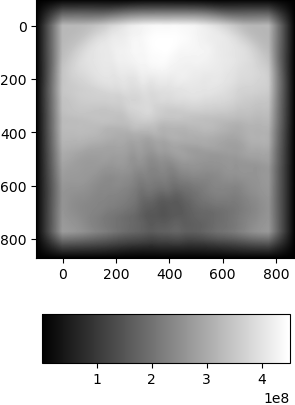
\includegraphics[width=\linewidth]{img/normalized_simple_corr}
		\caption{Simple cross--correlation of the (a) and (b) images}
		\label{normalized-simple-cross}
	\end{subfigure}
	\begin{subfigure}{.49\textwidth}
		\centering
		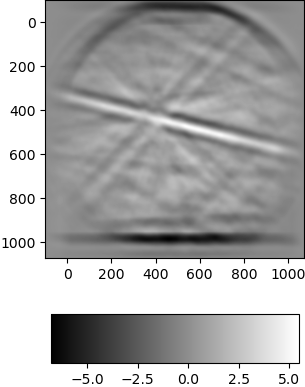
\includegraphics[width=\linewidth]{img/normalized_corr}
		\caption{Normalized cross--correlation of the (a) and (b) images}
		\label{normalized-cross}
	\end{subfigure}
	
	\caption{A comparison between the simple and zero--normalized cross--correlation. An image of backscatter pattern (a) is correlated with its subregion (b). (c) shows that simple cross--correlation is affected by varying brightness in different parts of images. (d) shows that normalization of the images improve the cross--correlation results.}
\end{figure}

That is why zero--normalized cross--correlation is used. It is based on subtracting respective means from each image. Normalized cross--correlation of two images $f$ and $g$ is defined as follows:
\[
\textsc{ZNCC}[i,j] = \sum_{x=-\infty}^{\infty}\sum_{y=-\infty}^{\infty} \frac{1}{\sigma_f \sigma_g}(f[x,y] - \mu_f)(g[x+i,y+j] - \mu_g),
\]  
where $\mu_f$ and $\mu_g$ are the means of the images and $\sigma_f$, $\sigma_g$ are their standard deviations. For an image $f$ with size $W \times H$, they are defined like so:
\begin{align*}
\mu_f &= \frac{1}{WH} \sum_{x,y}{}f[x,y], \\
\sigma_f &= \sqrt{\frac{1}{WH-1} \sum_{x,y}(f[x,y]-\mu_f)^2}.
\end{align*}

\Cref{normalized-cross} shows the zero--normalized cross--correlation of the figures \ref{normalized-initial} and \ref{normalized-pattern}. The area of the highest correlation is now clearly visible and corresponds to a Kukuchi line in the original image. Subtracting the mean of both images makes the algorithm less prone to brightness changes across the image.



The intuition behind this behavior is as follows. By the definition of simple cross--correlation, pixels with low brightness multiply and result in low correlation. After subtracting the means, low values in both images become negative. However, two negative numbers multiply into a positive value, so they increase the correlation. On contrary, very bright and very dull pixels multiply into a negative number so their difference causes that they lower the overall correlation value.

\section{Least squares}

The least squares method is used to approximate the solution of systems of equations do not have an exact solution, since there are more equations than unknowns. Such systems are also called overdetermined systems. In EBSP analysis, the least squares method is used to approximate coefficients of a quadratic function from its several known points.

In the first place, let us formulate the problem that the least squares method addresses. Let $n,m \in N, n > m; A \in \mathbb{R}^{n \times m}; x \in \mathbb{R}^m$ and $b \in \mathbb{R}^n$. Then $Ax = b$ is an overdetermined system of linear equations. It may have a solution, if $b$ is a linear combination of column vectors of $A$ ($b$ is in column space of $A$), but in general, that is not the case.

Instead of solving the system, we search for a vector $x'$ that has the least difference from the solution:
\[
x' = \min_x \norm{Ax - b},
\]
where $\norm{\cdot}$ denotes Euclidean norm. For a vector $x \in \mathbb{R}^n$, it is defined as:
\[
\norm{x} = \sqrt{\sum_{i=0}^{n} x_i^2}.
\]
So we minimize the sum of squared differences between the left and right sides of the equations in the system, hence the name least squares.

The least squares solution can be calculated using only matrix multiplication and inversion as follows (a proof can be found for example in \cite{anton2013elementary}):  
\[
x' = (A^TA)^{-1}A^Tb.
\]

This formula is not used in practice because of effectiveness and numerical stability (instead, it is better to solve the equation $A^TAx = A^Tb$). However, for the algorithm described in this thesis the matrix $A$ does not depend on the input data and thus it is possible to precompute the $(A^TA)^{-1}A^T$ matrix. That reduces the computation of the least squares vector to one matrix--vector multiplication.


\section{Algorithm description}

In the following section, we describe how are the zero--normalized cross--corre\-lation and the least squares mathod used to analyze the deformation of EBSPs.

As described in the beginning of this chapter, the algorithm we implement in this thesis takes deformed EBSPs and cross--correlates several regions of interest with a reference EBSP. A region of interest (ROI) is a rectangular part of an image defined by its size and position. The algorithm then finds the maximum of the cross--correlation, which yields the vector of deformation with one pixel accuracy. Finally, it improves the accuracy by finding the maximum of a fitted quadratic function.

The algorithm takes the following input:
\begin{itemize}
	\item reference EBSP image with size $W \times H$
	\item $N$ deformed EBSP images, each with size $W \times H$
	\item $M$ positions ROIs that will be compared from each image
	\item size $w \times h$ of each ROI
	\item size of neighbourhood $s \times s$ of the cross correlation maximum that will be used to fit the quadratic function
\end{itemize}
The result of the algorithm is a list of $M$ shifts for each of the $N$ deformed EBSPs (see \cref{roi-shifts:result} for visualization of the shifts for one EBSP).

Algorithm \ref{algo-whole} describes the whole process in pseudocode. It goes through all deformed EBSPs and all ROI positions specified in the input. For each ROI, it computes the zero--normalized cross--corre\-lation in three steps:
\begin{enumerate}
	\item Find means of the ROI
	\item Subtract the means from ROIs
	\item Compute cross--correlation
\end{enumerate}
The result is an image (two--dimensional array) with size $(2w-1) \times (2h-1)$.

\begin{algorithm}
	\caption{EBSP deformation processing}
	\label{algo-whole}
	\KwIn{one reference EBSP \newline
		N deformed EBSPs \newline
	 	position of M regions of interest (ROI) from each EBSP \newline
 		size of one ROI \newline}
	\KwOut{deformation shifts for all M ROIs from all N deformed EBSPs}
	\vspace{5px}
	
	refEBSP  $\leftarrow$ load reference EBSP from disk\;
	\ForEach{deformed EBSP}{
		defEBSP $\leftarrow$ load EBSP from disk\;
		\ForEach{\emph{roiPos} in ROI positions}{
			refROI, defROI $\leftarrow$ extract ROI from refEBSP and defEBSP\;
			
			find the mean of both ROIs and subtract it\;
			
			crossResult $\leftarrow$ cross--correlate(refROI,defROI)\;
			%
			maxX, maxY $\leftarrow$ subpixelPeak(crossResult)\;
			output [maxX, maxY]\;
		}
	}
	
	\SetKwProg{Fn}{Function}{}{end}
	\SetKwFunction{FSubpixelPeak}{subpixelPeak}    
	\Fn{\FSubpixelPeak{crossResult}}{
		[maxX, maxY] $\leftarrow$ argmax(crossResult)\;
		neigh $\leftarrow$ extract neighborhood of [maxX, maxY]\;
		
		fit a quadratic function to neigh using the least squares method\;
		\KwRet maximum of the quadratic function\;
	}
\end{algorithm}

\subsection{Subpixel peak}

Next, we find the maximum of the cross--correlation. The location of the maximum $[x,y]$ in the matrix is the shift between the deformed and reference ROI. However, the precision of one pixel is not enough because it is too big in comparison with the nanoworld the EBSP technique studies. That is why we use the cross--correlated data to estimate the maximum with subpixel accuracy.

We take a square--shaped neighborhood of the maximum with size $s \times s$ and fit a two--dimensional quadratic function defined as:
\[
f(x,y) = a + bx + cy + dx^2 + exy + fy^2,
\]
where $a, b, c, d, e, f \in \mathbb{R}$. To fit such function is to estimate the 6 coefficients $a \dots f$. From the known points of the neighborhood $N$ of size $s \times s$, it is possible to create the following system of equations:
\[
\forall [x,y] \in \{0,1,\dots , s-1\}^2 : a + xb + yc + x^2d + xye + y^2f = N[x,y],
\]
where $a \dots f$ are unknown variables.

We have $s^2$ known points, from which we create $s^2$ equations. Since we have 6 unknown variables, $s$ has to be at least 3, so we have more equations than unknowns. 

We solve the system using the least squares method, which estimates the coefficients $a \dots f$. That means we know the equation of the quadratic function which fits the neighborhood.

\subsubsection{Subpixel peak example}

For instance, let $s$ be 3 and $N$ be the neighborhood of the maximum:
\[
N =
\begin{bmatrix}
751 & 819 & 765 \\
825 & 934 & 810 \\
768 & 798 & 725
\end{bmatrix}.
\]
Then, the linear system looks like this:
\[
\begin{bmatrix}
1 & 0 & 0 & 0 & 0 & 0\\
1 & 1 & 0 & 1 & 0 & 0\\
1 & 2 & 0 & 4 & 0 & 0\\
1 & 0 & 1 & 0 & 0 & 1\\
1 & 1 & 1 & 1 & 1 & 1\\
1 & 2 & 1 & 4 & 2 & 1\\
1 & 0 & 2 & 0 & 0 & 4\\
1 & 1 & 2 & 1 & 2 & 4\\
1 & 2 & 2 & 4 & 4 & 4
\end{bmatrix}
\cdot
\begin{bmatrix}
a \\ b \\ c \\ d \\ e \\ f
\end{bmatrix}
=
\begin{bmatrix}
751 \\ 819 \\ 765 \\ 825 \\ 934 \\ 810 \\ 768 \\ 798 \\ 725
\end{bmatrix}.
\]
The left side contains all the points from the set $\{0,1,2\}^2$; right side contains all the corresponding values from neighborhood $N$.

\subsubsection{Maximum of fitted function}

The last step in the algorithm is to find the maximum of the quadratic function. We do that using standard methods of mathematical analysis: we find where are the partial derivations of the function equal to zero.

The partial derivations of the quadratic function are:
\begin{align*}
\frac{\partial f}{\partial x}(x,y) &= 2dx + ey + b,\\
\frac{\partial f}{\partial y}(x,y) &= ex + 2fy + c.
\end{align*}

If the function has an extreme, then it is located at the point where the partial derivations are both zero. That implies the a linear system of equations with the following solution:
\begin{align*}
x_m &= \frac{2bf - ce}{e^2 - 4df}\\
y_m &= \frac{2cd - be}{e^2 - 4df}
\end{align*}

The point $[x_m, y_m]$ is the maximum of the function fitted to the neighborhood of the cross--correlation maximum. All that is left is to combine those two to get the offset of one ROI of the EBSP.
